\section{B-Splines}

B-Splines are in many ways a improvement over Bezier curves. They give us control over the continuity and allow for local support only. Cubic B-Splines are the most popular type, but we can define them for arbitrary degree. \medskip

A B-Spline $s(u)$ is built from piecewise polynomial bases and a sequence of knots $u_0 < u_1 < ...$
$$s(u) = \sum_{i = 0}^k d_i N^n_i(u)$$ 

They have the following properties:
\begin{itemize}
	\item \textbf{Partition of Unity}: $\sum_i N_i^n(u) = 1$
	\item \textbf{Positivity}: $N_i^n (u) \geq 0$
	\item \textbf{Compact support}: $N_i^n(u) = 0, \; u \not \in [u_i, u_{i+1}]$
	\item \textbf{Continuity}: $N_i^n$ is (n-1) times continuously differentiable
\end{itemize}

The basis functions are defined as:
$$N_i^n (u) = (u - u_i) \frac{N_i^{n-1}(u)}{u_{i+n} - u_i} + (u_{i+n+1} - u) \frac{N_{i+1}^{n-1}(u)}{u_{i+n+1} - u_{i+1}}$$
\subsection{Tensor Product Surfaces}

Getting from a curve to a surface involves taking a tensor product (outer product). Given two Bezier curves $b^m(u)$ and $b^n(v)$ we can create the surface: 
$$b^{m,n}(u,v) = \sum_{i=0}^m \sum_{j=0}^n b_{i,j} B_i^m(u) B_j^n(v)$$
\begin{center}
	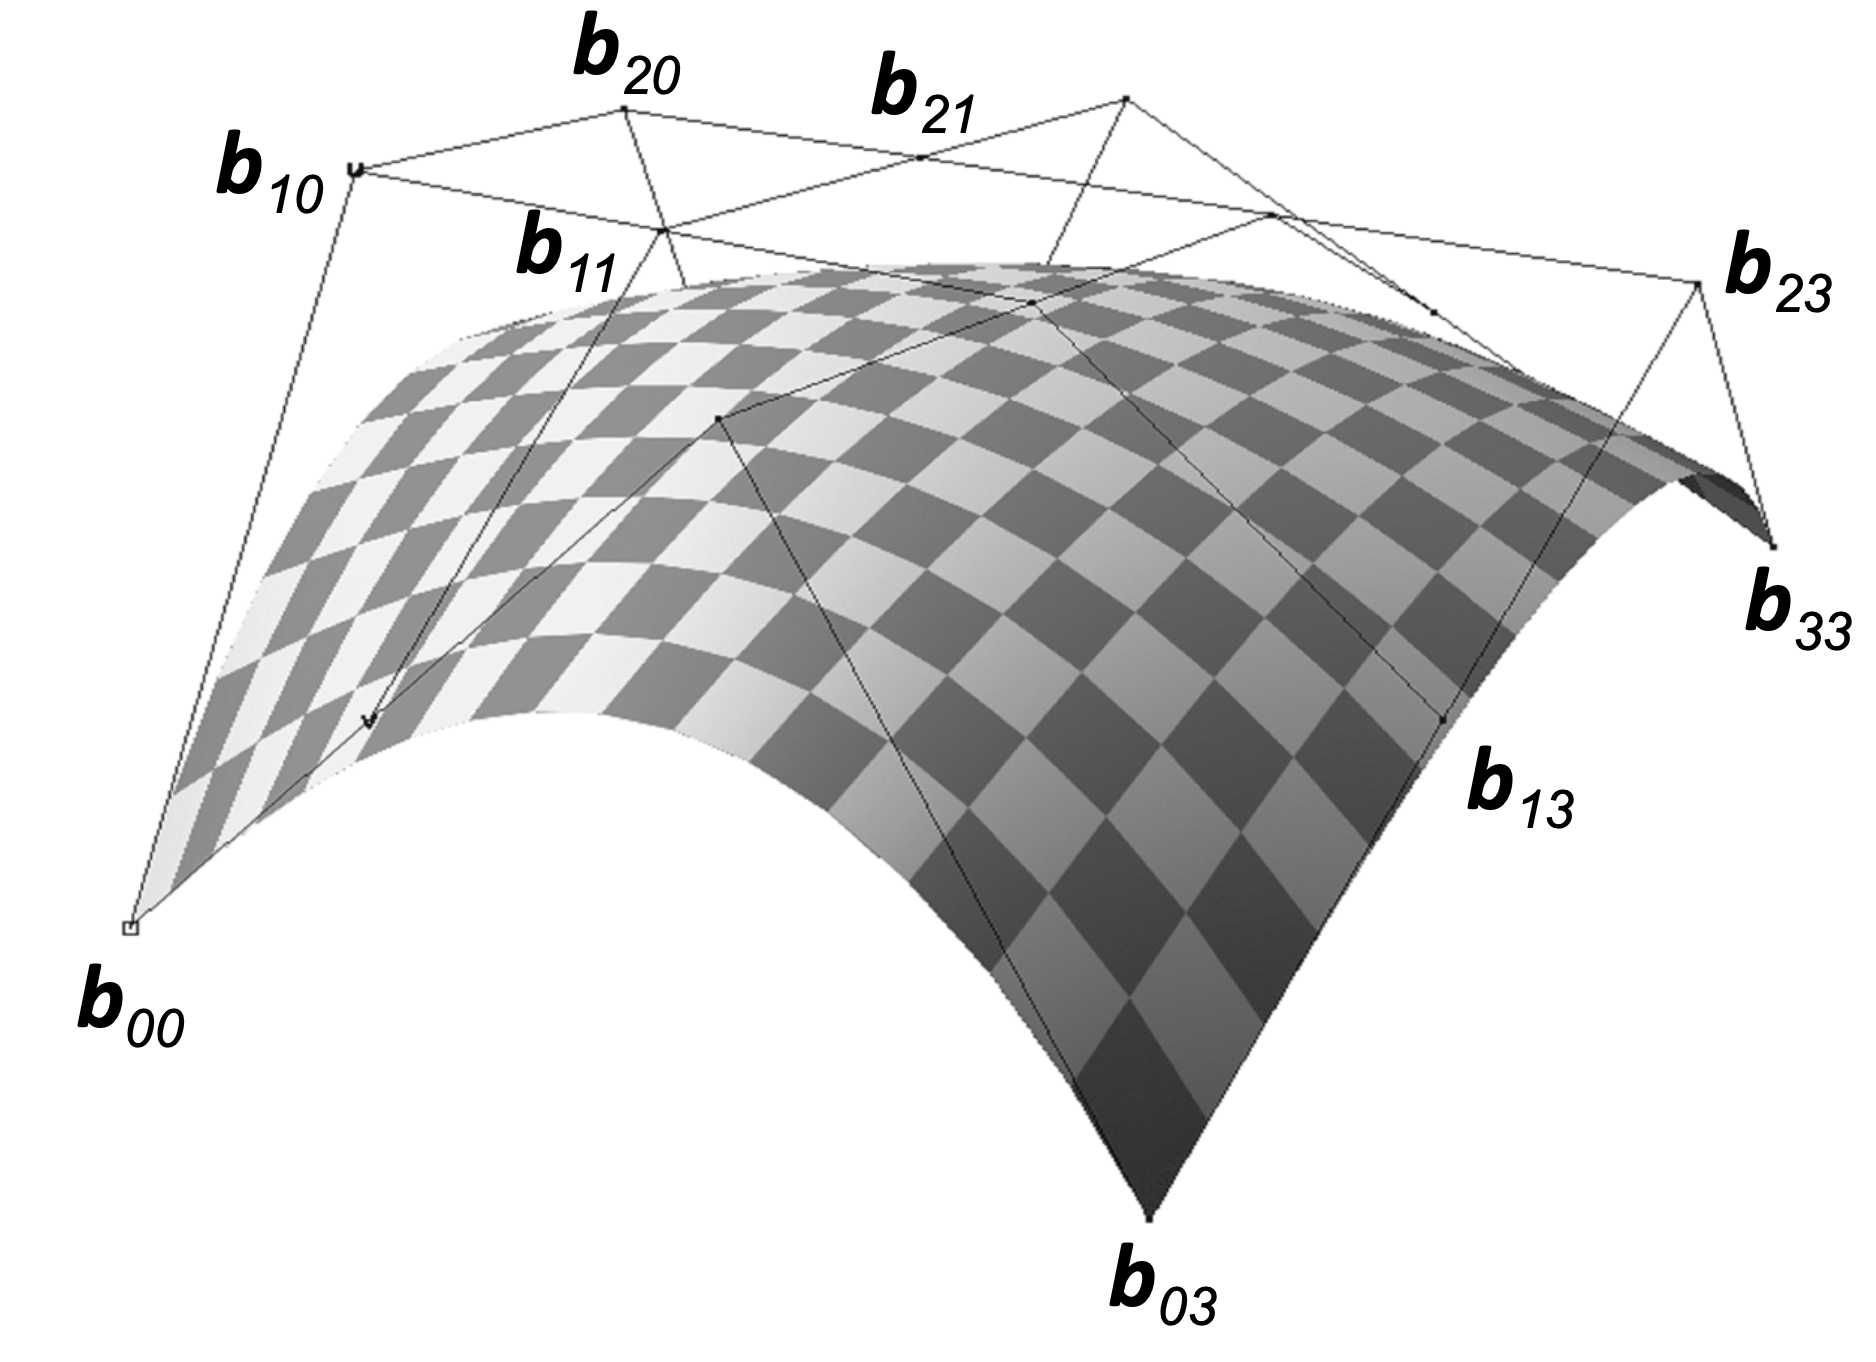
\includegraphics[width=0.9\linewidth]{bezier_surface.png}
\end{center}
